\documentclass{article}


% load package with some of the available options - you may not need this!
\usepackage[framed,autolinebreaks,useliterate]{mcode}
% for checklist
\usepackage{enumitem,amssymb}
\newlist{todolist}{itemize}{2}
\setlist[todolist]{label=$\square$}
\usepackage{pifont}
\newcommand{\cmark}{\ding{51}}%
\newcommand{\xmark}{\ding{55}}%
\newcommand{\done}{\rlap{$\square$}{\raisebox{2pt}{\large\hspace{1pt}\cmark}}%
\hspace{-2.5pt}}
\newcommand{\wontfix}{\rlap{$\square$}{\large\hspace{1pt}\xmark}}


% something NOT relevant to the usage of the package.
\usepackage{graphicx}
\usepackage{url,textcomp}
\setlength{\parindent}{0pt}
\setlength{\parskip}{18pt}
\title{ECTA Homework 2\\Genetic Algorithms\\and\\TSP}
\author{\color{blue}Erick Kramer, Mihir Patil\\ \texttt{\color{blue}erick.romero@smail.inf.h-brs.de , mihir.patil@smail.inf.h-brs.de}}
% //////////////////////////////////////////////////

\begin{document}

\maketitle

\section{Assignment Description}
	\begin{enumerate}
		\item{Write a Genetic Algorithm to solve the Traveling Salesman Problem (TSP)}
		\begin{itemize}
			\item{All cities visited once, coming back to the start city}
			\item{100 largest cities in Germany (data files on LEA)}
			\item{Minimize the distance traveled}
		\end{itemize}
		\item{This time, to give you further insight into the inner workings of genetic algorithms we would like you to compare different mutation and crossover rates. Please use the plotting templates from the last weeks homework for your comparision. Use the parameters listed below for you comparision and explain the observed effects. Therefore please test and compare the effects of 4 different mutation rates and 4 different crossover rates.}
		\begin{itemize}
			\item{Mutation rates:}
			\item[-]{1/nCities\%}
			\item[-]{1\%}
			\item[-]{10\%}
			\item[-]{99\%}
			\item{Crossover rates:}
			\item[-]{1\%}
			\item[-]{10\%}
			\item[-]{80\%}
			\item[-]{99\%}
		\end{itemize}
		\item{Ensure a large enough sample for reliable results by repeating the experiments at least 30 times and reporting the median}
	\end{enumerate}


\section{The Assignment}

\subsection{Coding GA for TSP}
\begin{enumerate}
%-------------------------%
% Put your code here:

\item \textbf{Tournament Selection}
	\lstinputlisting[firstline=31, lastline=53]{my_selection_T.m}
	
\newpage

\item \textbf{Crossover}
	\lstinputlisting[firstline=33, lastline=80]{my_crossover_T.m}
	
\item \textbf{Mutation}
	\lstinputlisting[firstline=30, lastline=51]{my_mutation_T.m}
	
\item \textbf{Elitism}
	\lstinputlisting[firstline=26, lastline=38]{my_elitism_T.m}	
	
%-------------------------%
\end{enumerate}

\subsubsection{Comparing Algorithms}
\newpage

		\begin{figure}[h!]
		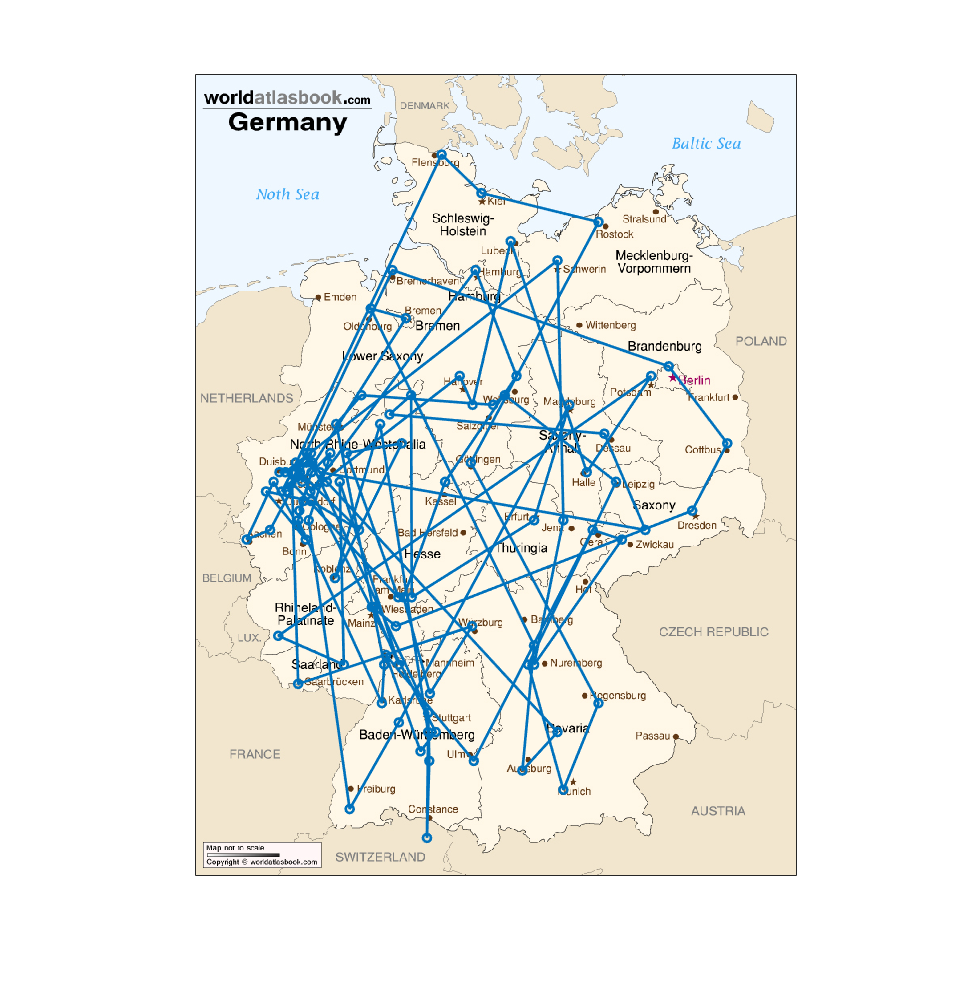
\includegraphics[width=0.5\textwidth]{img/one_point_30_runs_ind.png}
		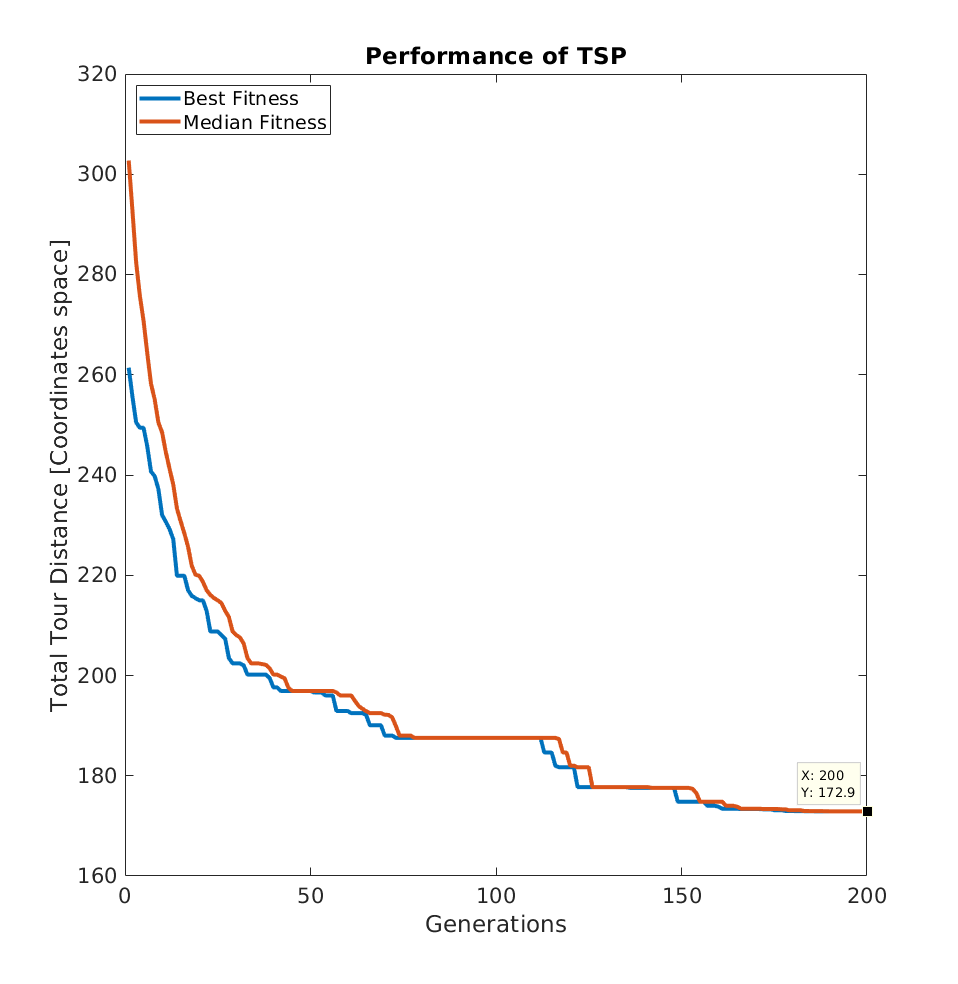
\includegraphics[width=0.5\textwidth]{img/one_point_30_runs_fit_med.png}
		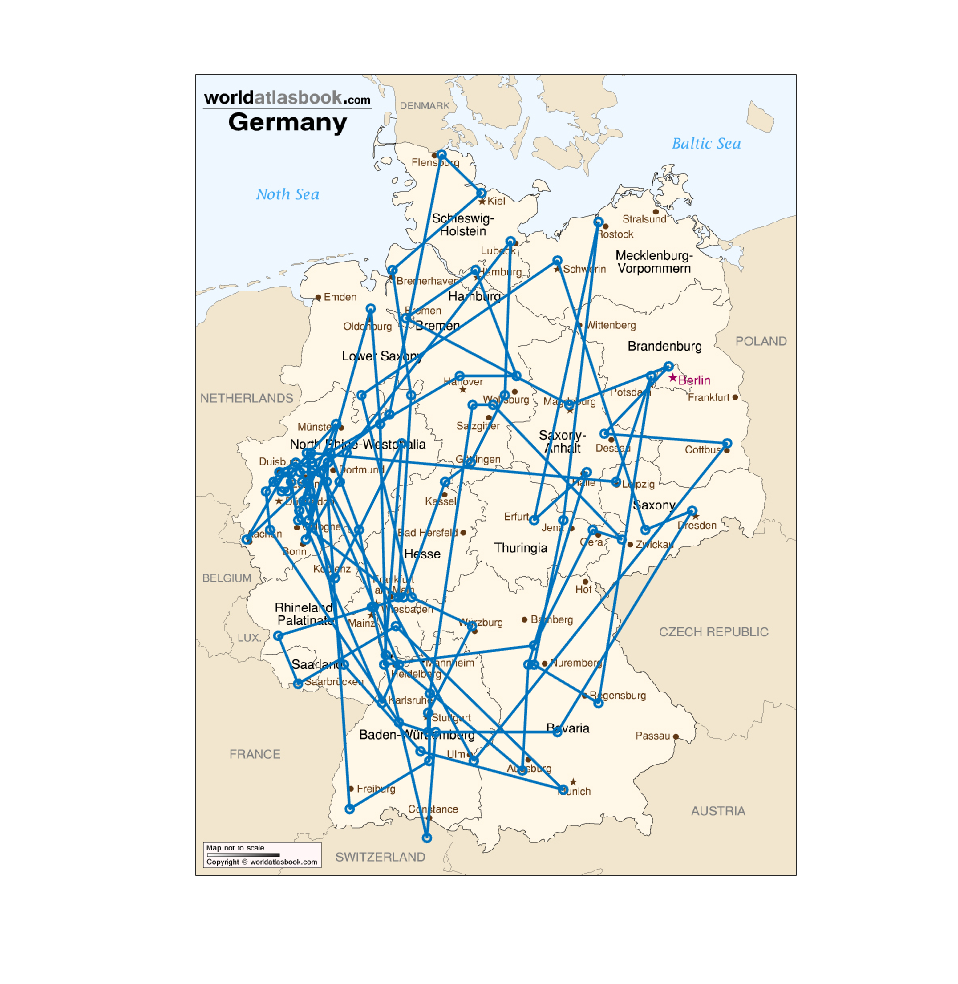
\includegraphics[width=0.5\textwidth]{img/two_points_30_runs_ind.png}
		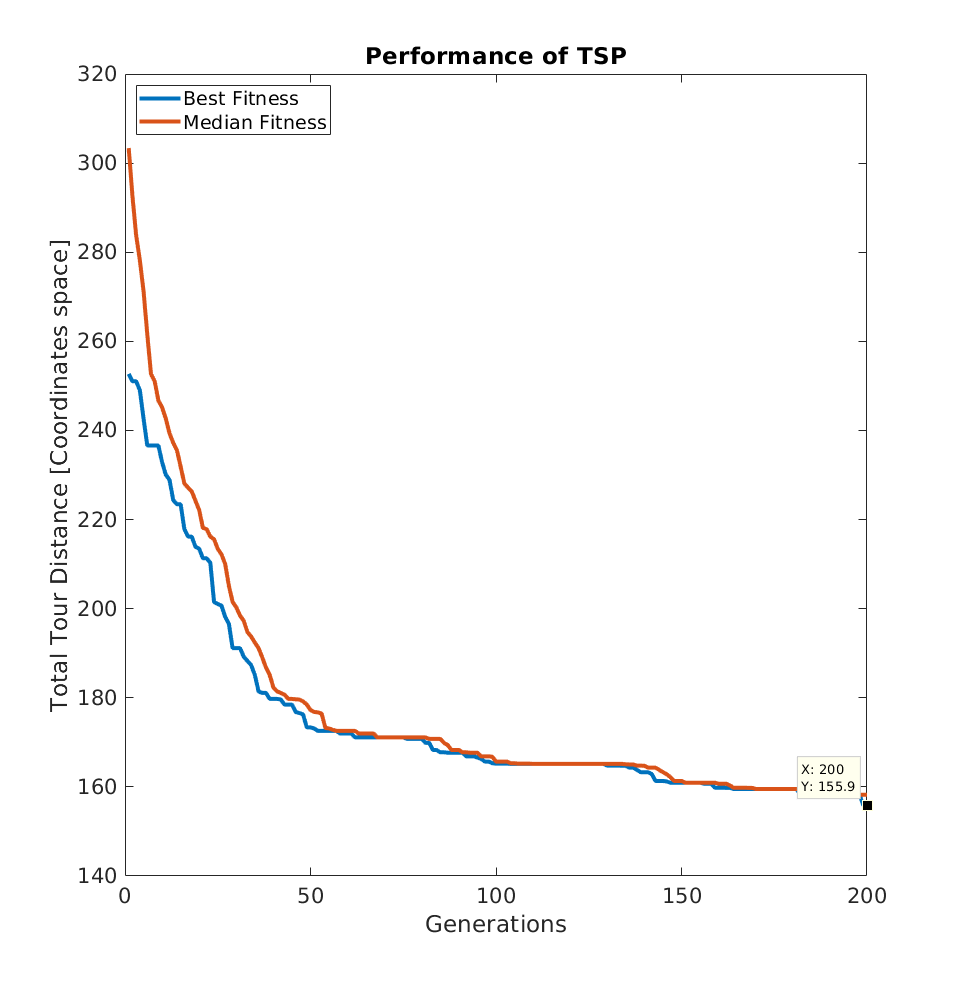
\includegraphics[width=0.5\textwidth]{img/two_points_30_runs_fit_med.png}
		\caption
		{
		\textbf{One point vs two point crossover with 30 runs}\newline
		\textit{Top Left:} One point crossover best individual,
		\textit{Top Right:} One point crossover fitness and median, 
		\textit{Bottom Left:} Two point crossover best individual, 
		\textit{Bottom Right:} Two point crossover fitness and median
		}
		\end{figure}
		
		\begin{figure}[h!]
		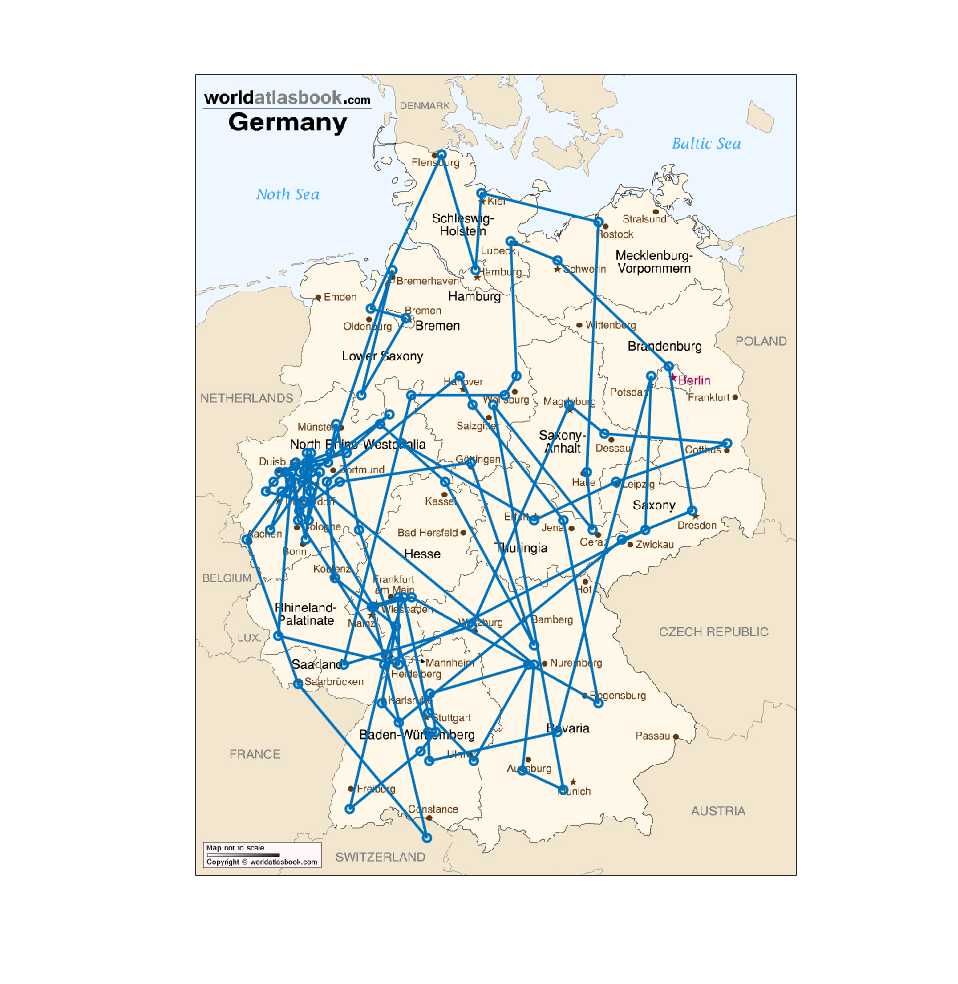
\includegraphics[width=0.5\textwidth]{img/cross_80_mut_10_ind.png}
		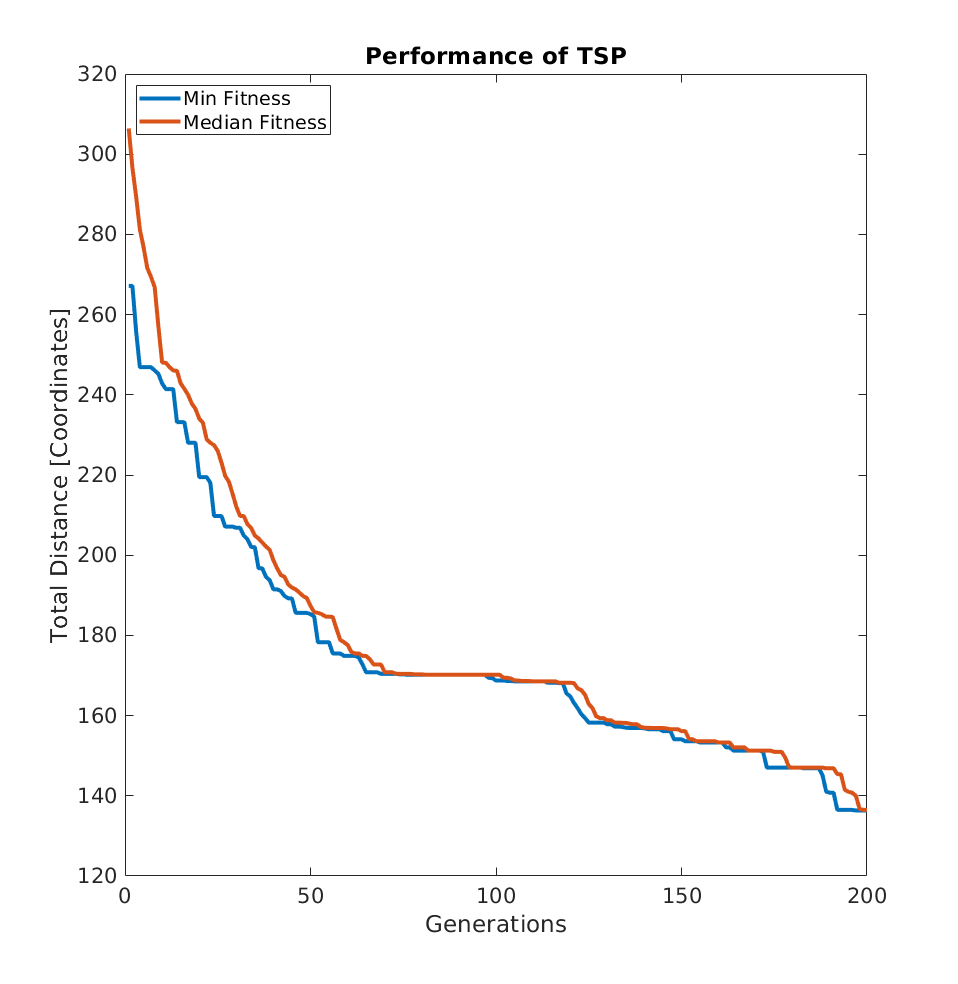
\includegraphics[width=0.5\textwidth]{img/cross_80_mut_10_fit_med.png}
		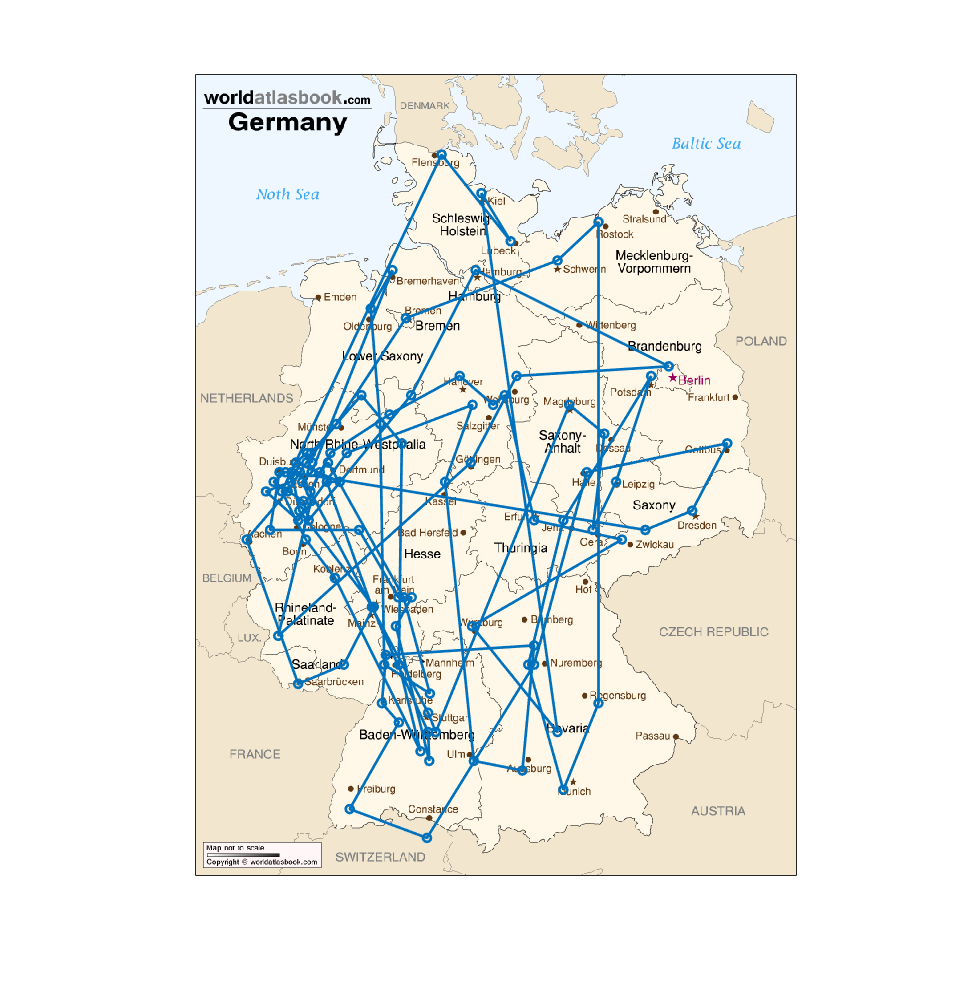
\includegraphics[width=0.5\textwidth]{img/cross_80_mut_10_ind_30_runs.png}
		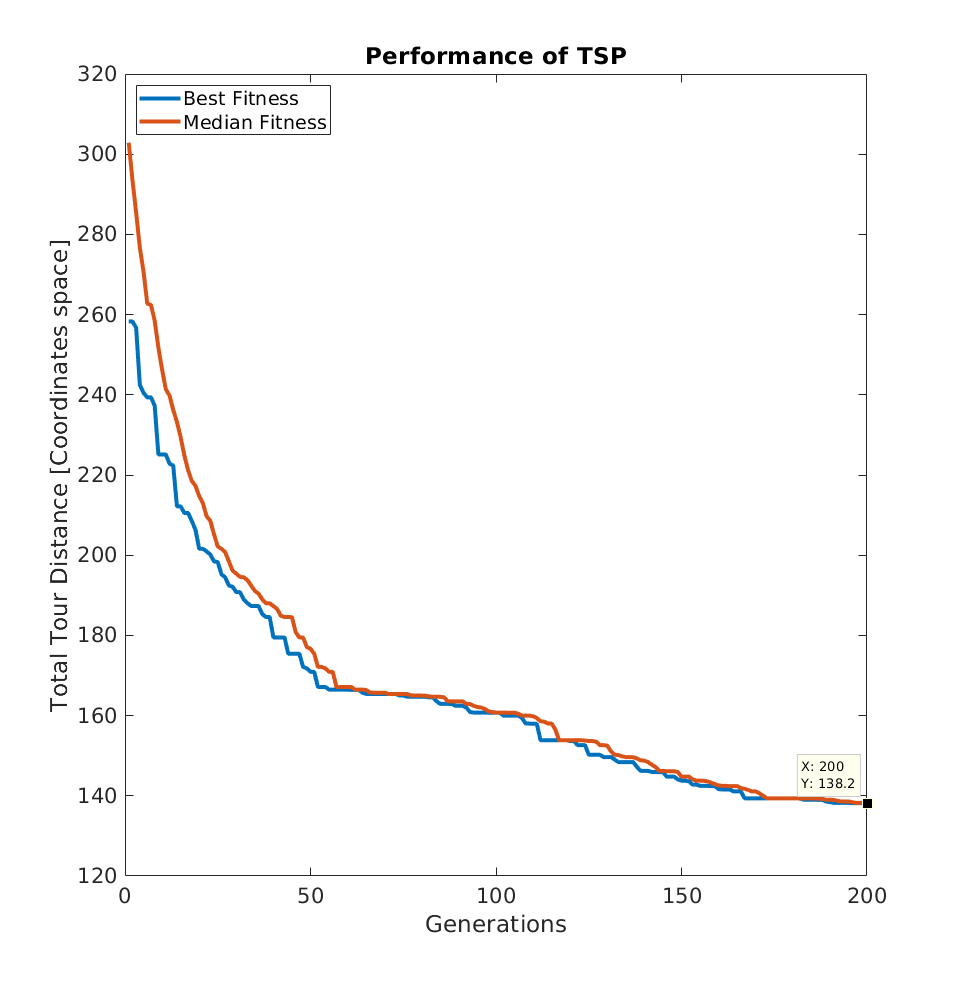
\includegraphics[width=0.5\textwidth]{img/cross_80_mut_10_fit_med_30_runs.png}
		\caption
		{
		\textbf{Best configuration mutation/crossover (80\% crossover, 10\% mutation) rate combination of single run vs 30 runs}\newline
		\textit{Top Left:} Single run best individual,
		\textit{Top Right:} Single run fitness and median, 
		\textit{Bottom Left:} 30 runs best individual, 
		\textit{Bottom Right:} 30 runs fitness and median
		}
\newpage
MIHIR: Insert explanation behind the different rates of mutation and crossover rates and why one works better than the other one.

\end{figure}

\end{document}